\documentclass[12pt,a4paper]{article}
\usepackage[margin=2.5cm,left=2cm,includefoot]{geometry}
\usepackage{hyperref}
\usepackage{array}
\usepackage{enumitem}
\usepackage{graphicx}
\usepackage[section]{placeins}
\usepackage{titlesec}

\setlength{\parindent}{0em}

\graphicspath{{Images/}}

% Header and footer
\usepackage{fancyhdr}
\pagestyle{fancy}

\rhead{COS 301}
\lhead{Team Objective C}
\fancyfoot{}
\fancyfoot[R]{Page \thepage}

\renewcommand{\headrulewidth}{2pt}
\renewcommand{\footrulewidth}{1pt}

\begin{document}

\begin{titlepage}
  \begin{center}
    \begin{figure}[t]
      \centering
      
\includegraphics[width=350px]{logo.PNG}
     \end{figure}
     
     \textsc{\LARGE COS301 Group Task 2 \newline \newline Architectural Design\\[0.5cm] Specifications}
     
     \textbf{\newline Team Objective C} \\
     \begin{flushright} \large
      Diana Obo \emph{u13134885}\newline
      Kamogelo Tsipa \emph{u13010931}\newline
      Linda Zwane \emph{u14199468}\newline
      Melvin Zitha \emph{u12138747}\newline
      Minal Pramlall \emph{u13288157}\newline
      Rotondwa Siavhe \emph{u????????}\newline
       \end{flushright} 
      \vfill %whitespace
      
      Team Objective C Github: \href{https://github.com/ShockwaveZA/Objective-C-Team}{Github} page.\\
      \url{https://github.com/ShockwaveZA/Objective-C-Team}
      
      \vfill
      {\large Date:}
      \\
      {\large \today}
     \end{center}
    \end{titlepage}


\tableofcontents
\newpage

\section{Design Constraints}
	\begin{itemize}
		\item The NavUp application must at least have basic navigation system functionalities.
		\item The location  of the user must be determined both indoors and outdoors.
		\item The NavUp system will be integrated into the Computer Science department's website.
		\item The NavUp system should allow the integration of a variety of services were navigation is the main objective.
		\item The NavUp application must only allow the administrator to create, update and delete information about events, venues and activities.
		
	\end{itemize}
    
\section{External Interface Requirements}
This section will cover the requirements of the external interface of the NavUP system. NavUP is going to be designed to operate as a mobile applications for smart devices such as smart phones and tablets; as such, the minimum requirements will fall in line with a typical entry-level smart device that is capable of running mobile applications.\newline

    \subsection{Minimum Requirements}
        \begin{itemize}
            \item 768x1024 minimum resolution
            \item Android, Apple or Windows Mobile Operating Systems
            \item WiFi enabled
            \item Internet coverage
        \end{itemize}
	
\section{UML}
	\subsection{UML - User}
	The architecture of the User group is decidedly much simpler than the other modules as the user module is characterized mainly by the Template Design Pattern.
	\begin{figure}[H]
		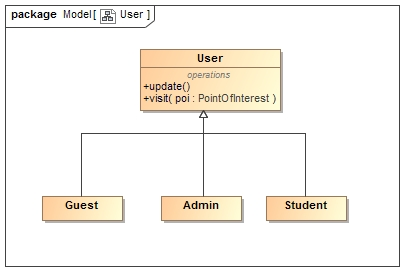
\includegraphics[width=\linewidth]{Images/User.jpg}
		\caption{UML of the User classes}
	\end{figure}
	
	\subsection{UML - Events}
	The modelling of the Events module will be characterized by the Observer design pattern, since the EventHandler will attach the users that are willing to participate, and will use the notify() method to communicate with only the participants of the event not a user that does not want to participate and just happens to be in proximity of event.
	\begin{figure}[H]
		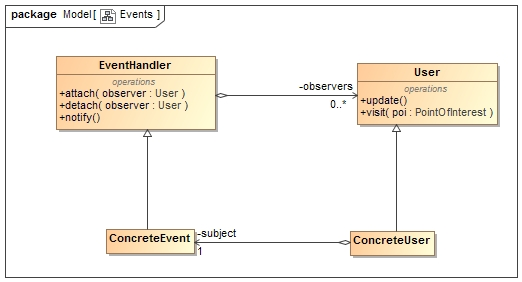
\includegraphics[width=\linewidth]{Images/Events.jpg}
		\caption{UML of the Events module}
	\end
	
	\subsection{UML - Fitness}
	The Fitness module, like Events, will also be using the Observer Design Pattern. The FitnessObserver will be used by Navigation to monitor the user and simply track the activity, rewarding the user by achieving milestones.
	\begin{figure}[H]
		\includegraphics[width=\linewidth]{Images/Fitness.jpg]
		\caption{UML of the Fitness module}
	\end{figure}
	
	\subsection{UML - Navigation}
	The Navigation module will make use of the Memento Design Pattern, the needs of this module is to save routes as well as perform remove and update operations. Memento best suits this need because of the Caretaker class that stores instances, or an entire route in this particular case.
	\begin{figure}[H]
		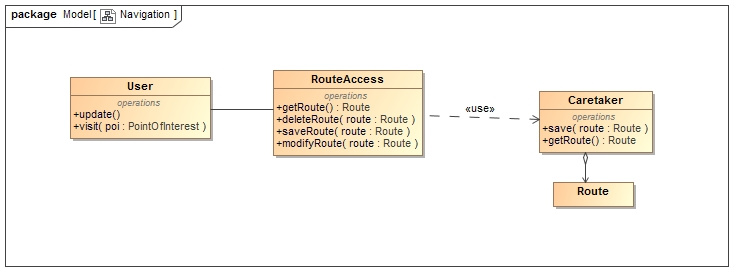
\includegraphics[width=\linewidth]{Images/Navigation.jpg}
		\caption{UML of the Navigation module}
	\end{figure}
	
	\subsection{UML - Points of Interest}
	The Points of Interest module will be using the Visitor Design Pattern, when a user is walking around and visits a point of interest, an event will be triggered. This event will provide the user with information of this point of interest and may also record that the user has visited this location in this instance (This may help with Surveillance).
	\begin{figure}[H]
		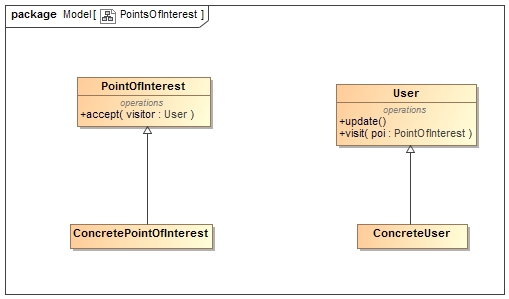
\includegraphics[width=\linewidth]{Images/PointsOfInterest.jpg}
		\caption{UML of the Points of Interest module}
	\end{figure}

\end{document}
